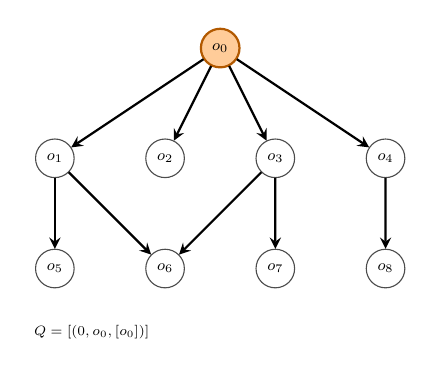
\begin{tikzpicture}[
    scale=0.7, transform shape,
    every node/.style={circle, draw, minimum size=7mm, font=\footnotesize\ttfamily},
    edge/.style={draw, ->, >=stealth, thick},
    current/.style={fill=orange!40, draw=orange!70!black, thick},
    default/.style={fill=white, draw=gray!60!black}
]
% Level 0
\node[current] (o0) at (3,4) {$o_0$};

% Level 1
\node[default] (o1) at (0,2) {$o_1$};
\node[default] (o2) at (2,2) {$o_2$};
\node[default] (o3) at (4,2) {$o_3$};
\node[default] (o4) at (6,2) {$o_4$};

% Level 2
\node[default] (o5) at (0,0) {$o_5$};
\node[default] (o6) at (2,0) {$o_6$};
\node[default] (o7) at (4,0) {$o_7$};
\node[default] (o8) at (6,0) {$o_8$};

% Edges from o0
\draw[edge] (o0) -- (o1);
\draw[edge] (o0) -- (o2);
\draw[edge] (o0) -- (o3);
\draw[edge] (o0) -- (o4);

% Edges from Level 1 to Level 2
\draw[edge] (o1) -- (o5);
\draw[edge] (o1) -- (o6);
\draw[edge] (o3) -- (o6);
\draw[edge] (o3) -- (o7);
\draw[edge] (o4) -- (o8);

% Queue annotation
\node[draw=none, rectangle, anchor=north west, align=left, font=\scriptsize, text=black]
    at (-0.5,-0.8) {$Q = [(0, o_0, [o_0])]$};
\end{tikzpicture}
